\chapter{Introduction}
\begin{figure}
\centering
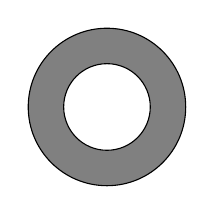
\begin{tikzpicture}[scale=.25]
  \filldraw[draw=black,fill=gray] (0,0) circle [radius=4];
      \filldraw[draw=black,fill=white] (0,0) circle [radius=2.2];
 \end{tikzpicture}      
 \hspace{.5cm}
\begin{tikzpicture}[scale=.25]
    \foreach[count=\p] \x / \y in \data { 
	\node[draw, circle, scale=.25, fill=white](\p) at (\x, \y) {};
    } 
 \end{tikzpicture}
 \caption{Point Cloud sampled from annulus}
 \end{figure}
Over the past twenty years \emph{topological data analysis} has been found to be very useful in understanding scientific data. The primary tools of the field: persistent homology and mapper have been used in a wide variety of applications, including image processing~\cite{cid-lbs-08}, material science~\cite{SW-measuring-shape}, and cosmology~\cite{cosmic-web}. Unlike traditional data analysis, in which one concerns itself with modeling physical phenomena from measurements on finite sets of samples, topological data analysis assumes that the input point cloud $X$ comes from an unknown underlying geometric space $Y$ embedded in yet some known larger ambient space $Z$. Topological data analysis then focuses on the recovery of the lost topology of $Y$ using information about $X$ and $Z$~\cite{c-tnd-09}. In this thesis we aim to make the primary tool for topological data analysis, persistent homology, computable for practitioners. To this end we investigate parallel algorithms for the computation of persistent homology. This implies providing a mechanism for decomposing a topological space, performing persistence computations on subspaces, and then gluing this information back together. For a topologist, this means exploiting the \emph{\mv principle}. The main contributions in this work are two new parallel algorithms, the first for computing homology via mayer-vietoris, and the second which improves and extends it to this result persistent setting. We connect the first procedure to \emph{spectral sequences} a manual calculation tool used for computing algebraic structures by hand. To this end we also introduce persistent homology with the language of spectral sequences.

The structure of the thesis as as follows. First, we introduce general background material on algebraic topology. Second, to introduce spectral sequences, we will derive persistent homology using the spectral sequence of a filtration. Next, we will show how one can leverage the \emph{\mv spectral sequence}, to compute ordinary homology in parallel. Instead of introducing this spectral sequence, we provide a description using the \mvb{} an analogous topological space. We take a brief digression to discuss the complexity of finding decompositions of a space which yield efficient parallel computation. Finally, we will show how to modify this construction to provide a parallel algorithm for persistence based on mayer-vietoris. Additionally we will show how one can derive upper bounds on the fill-in of these reduced matrices in terms of the quality of the cover. We will present experimental results which explore the efficacy of these techniques.

\section{Background}
Suppose someone asked you describe the shape of this point cloud. One might be inclined to propose that the point cloud looks quite disconnected. Indeed, the topology of a set of points in $\R^n$ is not all that interesting. Perhaps, however, if you were to squint your eyes, you might be inclined to describe the shape as something like an annulus. Persistence is a tool for modeling this phenomenon. As an example, for any \emph{metric space} $(X,d)$ and  $\epsilon > 0$ we can define a space: \[ M_\epsilon = \bigcup_{x \in X} B_{\epsilon}(x) \] where $B_{\epsilon}(x) = \{ y \mid d(x,y) < \epsilon\} $ is the \emph{ball of radius $\epsilon$ around x}. Notice that by varying the scale parameter $M_\epsilon$ has different topologies. The collection $\{M_\epsilon\}_\epsilon$ of spaces together with the inclusion maps between $M_\epsilon$ and $M_{\epsilon'}$ for any $\epsilon < \epsilon'$ is called a \emph{one parameter family} of spaces.   
 
 \begin{figure}
\centering
 \hspace{.5cm}
 \begin{tikzpicture}[scale=.25]
\begin{pgfonlayer}{ball}
      \foreach[count=\p] \x / \y in \data {
         \fill[gray!50,radius= .3 cm] (\x,\y) circle{};
	}
 \end{pgfonlayer}{ball}
	\foreach[count=\p] \x / \y in \data {
	 \node[draw, circle, scale=.25, fill=white](\p) at (\x, \y) {};
	 }
\end{tikzpicture}
 \hspace{.25cm}
\begin{tikzpicture}[scale=.25]
\begin{pgfonlayer}{ball}
      \foreach[count=\p] \x / \y in \data {
         \fill[gray!50,radius= .6 cm] (\x,\y) circle{};
	}
 \end{pgfonlayer}{ball}
	\foreach[count=\p] \x / \y in \data {
	 \node[draw, circle, scale=.25, fill=white](\p) at (\x, \y) {};
	 }
\end{tikzpicture}
 \hspace{.25cm}
\begin{tikzpicture}[scale=.25]
\begin{pgfonlayer}{ball}
      \foreach[count=\p] \x / \y in \data {
         \fill[gray!50,radius= 1 cm] (\x,\y) circle{};
	}
	\fill[gray!50,radius= 2.4 cm] (0,0) circle{};
 \end{pgfonlayer}{ball}
	\foreach[count=\p] \x / \y in \data {
	 \node[draw, circle, scale=.25, fill=white](\p) at (\x, \y) {};
	 }
\end{tikzpicture}
\caption{Model spaces at various scales}
\end{figure}

Persistent topology concerns itself with capturing topological features which can be found at multiple scales of a parameterized family of spaces.

\section{Preliminaries}
We begin with a review of algebraic topology. We refer the reader to Hatcher for further background material in algebraic topology~\cite{hatcher}.
\subsection{Topological Spaces \& Simplicial Complexes}
A topological space on a set $X$ is the pair $(X,T)$ where $T$ is a subcollection of $P(X)$, containing $\emptyset$ and $X$, and is further 
closed under countable unions, and finite intersections. 
Elements of $T$ are referred to as open sets. The complement of an open set is a closed set.

Some examples of topological spaces are, the $D^n$ the unit disk in $R^n$, $S^n$ the unit sphere in $R^{n+1}$. and $\partial D^n = S^{n-1}$ the boundary of the $n$-disk.  

A \emph{simplicial complex} is a collection $\K$ of finite sets called
\emph{simplices} such that if $\sigma \in \K$ and $\tau \subseteq \sigma$ then 
$\sigma \in \K$. We say that $\tau$ is a \emph{face} of $\sigma$, its \emph{coface}. A simplex
is \emph{maximal} if it has no proper coface in $\K$. The set of maximal cells of a 
simplicial complex $\K$ is $\M(\K)$. If $\card{\sigma} = k+1$
then $\sigma$ is a $k$-simplex, it has \emph{dimension} $k$, denoted 
$\dim{\sigma} = k$. We say that $\K$ is \emph{$d$-dimensional} if 
$d = \max_{\sigma \in \K} \dim{\sigma}$. A simplicial complex is a topological space, where the 
usual topology specified by specifying that a closed set is the closure of any simplex.

Suppose we have a subset $L \subseteq K$.  $L$ is a \emph{subcomplex}
if it is a simplicial complex. The \emph{closure} of $L$ is 1
$\Cl(L) = \{ \tau \mid \tau \subseteq \sigma \in L\}$ and it is a simplicial complex. The 
\emph{$k$-skeleton} of a complex $\K$ is the set of all simplices
of dimension less than or equal to $k$. Note that the 1-skeleton of
any complex is as a graph.

Let $\Delta^n$ be the standard $n$-simplex~\cite{hatcher}. For any
\emph{indexing set} $J \subseteq [n]$, $\Delta^J$ is the $(\card{J}-1)$ 
dimensional face of $\Delta^n$  that is defined on $J$. In the abstract setting we may
identify $\Delta^n$ with the set $[n] = \{1, \ldots, n\}$ of natural numbers, and $\Delta^J$ with the set $J$.

A simplicial complex may be viewed as the result of gluing simplices of 
different dimensions along common faces. Other types of complexes are defined 
similarly using different types of \emph{cells}. Such \emph{cellular} complexes include \emph{cubical} complexes, \emph{simplicial sets}. $\Delta$-complexes, and \emph{CW-complexes}, 
to name a few~\cite{ez-ssc-50,hatcher,kmm-ch-04,m-soat-68}. We end this section by defining finite dimensional CW-complexes.

 A finite dimensional CW-Complex $X$ is defined as the finite union $X = \bigcup_n X_n$, where $X_0$ is a given set of $0$-cells. One defines the $k$-cells $X_k$ inductively from $X_{k-1}$. To attach a $k$-cell $\sigma_\alpha$ construct an \emph{attaching map} $\phi_\alpha: S^{k-1} \rightarrow X_{k-1}$. We then define $X_k = X_{k-1} \sqcup D^k_\alpha / \sim$ where we quotient by the relation $x ~\sim \phi_\alpha(x)$ for $x \in \partial D^k_\alpha$. In practice we only consider the class of  \emph{computable CW complexes} which are finite dimensional CW-complexes with computable attaching maps.

\subsection{Maps, covers, and filtrations}
A map $f: X \rightarrow Y$ between topological spaces is \emph{continuous} if the inverse image of every (open/closed) set in $Y$ is (open/closed) in $X$. A pair of maps $f,g: X \rightarrow X$ are \emph{homotopic}, denoted $f \tilde g$, if there is a continuous map $F: X \times [0,1] \rightarrow X$ with $F(x,0) = f(x)$ and $F(x,1) = g(x)$. Two spaces are said to be \emph{homotopy equivalent}, denoted $X \sim Y$, if there exists maps $f: X \rightarrow Y$ and $g: Y \rightarrow X$ such that $f \circ g \sim 1_Y$ and $g \circ f \sim 1_X$.

If a space $X$ is \emph{contractible} if it is homotopy equivalent to a point.

Given a simplicial complex $\K$, An \emph{open cover} of $\K$ is a collection of subsets $\{\C_i\}_i$ of $\K$ where $K = \bigcup_i \C_i$. Similarly, we call a cover closed if each element of the cover is closed.

The \emph{nerve} $\N(\C)$ of a cover $\C$ is the simplicial complex on $[\card{\C}]$ whose $k$-simplices represent the non-trivial intersections of subsets of $\C$ of size $k+1$. The nerve may be regarded as a subcomplex of $\Delta^n$ and so we may denote its simplices by $\Delta^J$ where $J \subseteq [\card{\C}-1]$.

Let $\K$ be any topological space $\C$ be an cover of it, and $\N$ be the nerve of $\C$. If every element of $\C$, as well as all non-empty intersections of elements in $\C$, are contractible, then $\N$ is homotopy equivalent to $\K$. This is the \emph{Nerve Lemma}~\cite{hatcher}.

Recall from the previous section that a sequence of spaces connected by continuous maps is referred to as a one-parameter family. Let $M = \{M_\epsilon\}$ be the one-parameter family defined in the previous section. Let $\C = \{\C_\epsilon\}$ be the collection of open sets in $\R^n$, defining every member of $M$. We may define another one parameter family $\{ \N_\epsilon \}$ where $\N_\epsilon$ is the nerve of $\C_\epsilon$. Observe that whenever $\epsilon < \epsilon'$ there is an inclusion map: $\N_\epsilon \rightarrow \N_{\epsilon'}$.

We now redefine $N_{\epsilon}$ geometrically. Specifically we define the \emph{Cech}-Complex at scale $\epsilon$ as the set:
\[ C_\epsilon = \{ [ x_0, \ldots x_k] \mid \bigcap_i B_\epsilon(x_i)  \neq \emptyset \}. \]
Unfortunately, determining membership in $C_\epsilon$ can be quite complicated. A simpler, construction is the Vietoris-Rips complex:
\[ V_\epsilon = \{ [x_0, \ldots x_k] \mid d(x_i, x_j) < \epsilon \textrm{ for all } i,j  \}. \]

These two simplicial complexes are related. The following result is due to Ghrist \& DeSilva.
\begin{theorem}
\[ C_\epsilon \rightarrow V_\epsilon \rightarrow C_{2\epsilon} \]
\end{theorem}
\begin{proof}
See $\cite{ghrist-n-desilva}$
\end{proof}

We define a \emph{filtration} of topological spaces to be a finite sequence of topological spaces connected by
continuous maps. Given a filtration of simplicial complexes, whose final space is $\K$ we can create a  
partial ordering on the simplices of $\K$ such that the $i^{th}$ prefix of the ordering is the image in $\K$ of the $i^{th}$ map. Each prefix is itself a sub complex of $\K$, so in practice we consider only filtrations of spaces connected by inclusion maps.

\section{Algebra}
In this section we provide a review of algebra. An \emph{abelian group} $(S,+)$ is a set $S$ together with an associative, commutative binary operation $+: S \times S \rightarrow S$, which has:
\begin{itemize}
\item[additive identity] a element $0$, such that for each $s \in S$, $s+0 = 0+s = 0$.
\item[additive inverse] For each element $s \in S$, an element $t$ such that $s+t = 0$.
\end{itemize}
\begin{example}
The set $\Z$ of integers are a group under the operation of addition. The set of all invertible $n \times $ matrices, are a group, the \emph{general linear group}.
The set $\Z_n$ of integers modulo $n$ is a group under addition modulo $n$.
\end{example}
A \emph{commutative ring with unit} $(S,+,\cdot)$ is an abelian group $(S,+)$  together with another associative, commutative, binary operation $\cdot$ for which:
\begin{itemize}
\item[distributivity] for all $a,x,y \in S$ $a \cdot (x + y)  = a \cdot x + a \cdot y$ 
\item[multiplicative identity] $1 \in S$ such that for all $s \in S$ $1 \cdot s = s \cdot 1 = s$. 
\end{itemize}
In this work all rings are considered to be a commutative ring with unit, unless otherwise specified.  
\begin{example}
$\Z$, $\Z_n$, $\Q$, $\R$ and $\C$ are rings. Another important example is the set $R[t]$ of polynomials in $t$ which coefficients in any other ring $R$.
\end{example}
A \emph{field} $F$ is a ring which further has \emph{multiplicative inverses}.
\begin{example}
$\Q$, $\R$ and $\C$ are rings.  $Z_n$ is a field whenever $n = p^k$ for some prime $p$ and $k > 0$.
\end{example}
An \emph{ideal} $I$ of a ring $R$ is an additive subgroup with the following additive property:
\[ \textrm{ for each } x \in I, \textrm{ and each } r \in R, x \dot r, r \cdot x \in I  \]
And ideal $I$ is \emph{principal} if for some $a \in I$, we have: $I = Ra \{ ra \mid r \in R\} = \langle a \rangle$.
A ring $R$ is an \emph{principal ideal domain} if every ideal in $R$ is principal.
\begin{example}
$\Z$, $\Z_n$, $\Q$ $\R$ and $\C$ are principal ideal domains. $\Z[x]$ is not a principal ideal domain. $R[t]$ is a principal ideal domain if and only if $R$ is a field. However
even over fields $R[x,y]$ the ring of polynomials in two variables is not a principal ideal domain.
\end{example}
For any ring $R$ an \emph{R-module} $M$ is an \emph{abelian group} together with an associative, scalar multiplication by $R$: 
\begin{itemize}
\item[distributivity] for all $r \in R$ and $x,y \in M$ $a \cdot (x + y)  = a \cdot x + a \cdot y$
\item[identity] $1_R \cdot x = x$
\end{itemize}
In particular, when $R$ is a field $k$, the concept of $k$-module and $k$-vector space are identical.
\begin{example}
Any ring is a module over itself.  All groups are $\Z$-modules. $R[t]$, the ring of polynomials with coefficients in a ring $R$, is an $R$-module. If $S$ is any set and $M$ is any $R$-module, then the collection of linear functions from $S$ to $M$, denoted $M^S$, is an $R$-module where the action $(rf)(s) =  r \cdot f(s)$.
\end{example}
Given two $R$-modules $M$ and $N$ there are the \emph{direct sum} of modules $M \oplus N = \{ (m,n) \mid m \in M and n \in N \}$.
An $R$-module $N$ is said to be a \emph{direct summand} of $M$ if $M = N \oplus E$ for some $R$-module $E$. 
A \emph{submodule} $N$ of an $R$-module $M$ is a subset of the module that is itself an $R$-module. Clearly, all summands are submodules, but the converse is not true.
If a module $M$ is said to be \emph{decomposable} if it can be written as a direct sum of two non-trivial summands, modules which are not decomposable are \emph{indecomposable}. 
\begin{theorem}
Any(?) finitely generated $k[x_1, \ldots x_n]$-module can be decomposed into indecomposables in polynomial time in the description of the module. 
\end{theorem}
A \emph{module homomorphism} is a group homomorphism respecting scalar multiplication. Given an $R$-module homomorphism $f: X \rightarrow Y $, we define the \emph{kernel} of $f$, the \emph{image} of $f$ and the co-kernel of $f$, as follows: 
\begin{itemize}
\item $\ker{f} = \{ x \mid f(x) = 0 \}$. 
\item The \emph{image} of $f$ $\Im{f} = \{ f(x) \mid x \in X\}$, 
\item The \emph{co-kernel} of $f$ = $Y/\Im{f}$.
\end{itemize}
Module homomorphisms provide two more important example of $R$-modules. That is if $M$ and $N$ are $R$-modules then the set $\operatorname{Hom}(M,N)$ of $R$-module homomorphisms, is itself an $R$-module under addition of functions, and the obvious scalar multiplication. Now suppose that $\{M_i\}$ are a sequence of $R$-modules connected by module homomorphisms. Certainly there is an $R$-module structure on $M = \bigoplus M_i$, but there is also a $R[t]$-module structure, where the action of $t$ on an element in $M_i$ applies the map $f_i$. Such a module is referred to as a \emph{graded module}.

\subsection{Homology}
In this section, we describe the homology of cellular spaces. 
Suppose we are given a finite cellular complex $\K$ and a ring $R$. 
The \emph{$d$th chain of space $C_d$} is the $R$-module generated by 
the set of $d$-dimensional cells of $K$, its \emph{canonical basis}.  
Suppose we are given a linear \emph{boundary operator} 
$\bd_d\colon C_d \rightarrow C_{d-1}$ such that 
$\bd_d \circ \bd_{d-1} \equiv 0$ for any $d$.  
The boundary operator connects the chain vector space into a 
\emph{chain complex $C_*$}:
\begin{equation*}
  \cdots \rightarrow             C_{d+1}
         \xrightarrow{\bd_{d+1}}  C_d
         \xrightarrow{\bd_d}     C_{d-1}
         \rightarrow \cdots .
\label{eqn:chaincomplex}
\end{equation*}
Given any chain complex, the \emph{$d$th homology module $H_d$} is:
\begin{equation}
  \label{eqn:homology}
  H_d = {\ker{\bd_d}}\,/\,{\im{\bd_{d+1}}}, 
\end{equation}
where $\ker(.)$ and $\im(.)$ are the \emph{kernel} and \emph{image} of $\bd$, 
respectively.
When $R$ is a field $k$ then each homology module is characterized fully by its \emph{Betti number}, 
$\betti_d = \dim{H_d}$. 
We now only need to define boundary operators to define homology. 
For simplicial homology, we begin by defining the action of the boundary operator on any
$n$-simplex $[v_0,\ldots,v_n] \in \K$:

\begin{equation*}
\bd_n [v_0,\ldots,v_n] = \sum_i (-1)^i [v_0,\ldots,\hat{v_i},\ldots,v_n],
\end{equation*}
where $\hat{v_i}$ indicates that $v_i$ is deleted from the vertex 
sequence. The boundary operator is the linear extension of the above action.

An important property of homology is \emph{functorality} namely whenever we have a continuous map $f: X \rightarrow Y$ between topological spaces there is an induced linear map $\tilde{f}$ between there homology vector spaces in any dimension. That is the following diagram commutes:
\[ \begin{tikzcd}
X \arrow{r}{f}\arrow{d}{H_d} & Y \arrow{d}{H_d} \\
H_d(X) \arrow{r}{\tilde{f}} & H_d(Y)
\end{tikzcd} \]
The map is defined as follows: First we define the \emph{induced chain map} $f_\sharp$ as the linear extension of the following action: 
\[ f_\sharp([v_0, \ldots v_d]) = 
\begin{cases} 
    [f(v_0) \ldots, f(v_d)] \textrm{ unless } f(v_i) = f(v_j) \textrm{ for some } i,j \\
    0 \textrm{ otherwise. }
   \end{cases}
\]
Then for any $[x] \in H_d(X)$ we have $\tilde{f}([x]) = [f_{\sharp}(x)]$.  That this map is well defined follows from 
the following lemma:
\begin{lemma}
$f_\sharp$ commutes with the $\partial$ operator. 
\end{lemma}
\begin{proof}
Assume first that $f(v_i) \neq f(v_j)$ for $i \neq j$.
\begin{align*}
f_\sharp(\partial([v_0, \ldots v_d])) &= \\
&= f_{\sharp}(\sum_i (-1)^i[v_0 \ldots \hat{v_i} v_d])  \\
&=  \sum_i(-1)^i [f_{\sharp}(v_0) \ldots \hat{f_{\sharp}(v_i)} f_{\sharp}(v_d)] \\
&=  \partial(f_\sharp([v_0, \ldots v_d]))
\end{align*}
Observe now that if there is more than two repeated elements, that the result holds trivially as all terms are zero. If there are exactly two repeated elements, then they appear
in the sum with opposing signs.
\end{proof}

If $X$ is a simplicial complex and $A$ is any subcomplex we define the \emph{relative homology} of $X$ by $A$ as $H_d(X,A) = H(C_d(X)/C_d(A))$. We will write $C_d(X,A)$ to refer to $C_d(X)/C_d(A)$. Note, some authors provide an alternative definition of $C_d(X,A)$ which is isomorphic to the definition stated here.

\subsection{Computing Homology}
Over field coefficients, homology is a vector space characterized by its dimension, so we may compute homology using \emph{Gaussian Elimination}. However, when the coefficient ring is taken to be an \emph{principal ideal domain}, we may use a similar technique, known as the \emph{Smith Normal Form}~\cite{uhlig}. Smith Normal Form, is a matrix reduction technique similar to Gaussian Elimination~\cite{uhlig}. This algorithm was written down in western mathematical literature by Smith~\cite{smith}, and then republished four decades later by Poincare~\cite{poincare-smith}. Of course, as previously mentioned this is a variant of Gaussian Elimination, which was known to the Chinese mathematical community in $\approx$ 100AD~\cite{chinese-ge}.

The smith normal form of an $m \times n$ matrix $M$ over a principal ideal domain $R$, is a factorization $M = SDU$ where $S$ and $U$ are invertible $m \times m$ and $n \times n$ matrices respectively, and $D$ is a diagonal matrix, of the same shape as $M$. Note that neither $S$ nor $U$ is unique. The nonzero diagonal entries of $D$ are entries in $R$. In the case that $M = \partial_k$ the $k^{th}$  boundary operator, we have that $d_i \mid d_{i+1}$. If $d_1, \ldots d_r = 1$, then $\betti_k = \dim(H_k(X)) = r$. The remaining nonzero elements of $D$ are referred to as \emph{torsion}. If $R$ is a field then there is no torsion elements. 
\begin{figure}
\begin{codebox}
\Procname{\proc{SMITH}($\partial$):}
\li $S \gets \partial$, $U \gets I$
\li $D \gets 0$
\li \For{columns $R_i$} 
\li \Do 
\li \While{$R_i \neq 0$ and $\exists j < i$ with $\operatorname{Lowest}[R_i]= \operatorname{Lowest}[R_j]$}
\li \Do
\li   $R_i \gets R_i - R_{ij}\alpha^{-1}_{ij}R_j$
\li   $U[j,i] \gets R_{ij}\alpha^{-1}_{ij}$
    \End
\li   $\tau \gets \operatorname{Lowest}[R_i]$
\li   $D_{ii} \gets R_{i,\tau}$
\li   $R_{i} \gets D_{ii}^{-1}R_{i}$
\End
\end{codebox}
\caption{Standard Reduction algorithm}
\label{alg:smith}
\end{figure}

We present an algorithm for computing the smith normal form in Figure~\ref{alg:smith}. Given a column $c$ the function $\operatorname{Lowest}[c]$, 
returns the position of the nonzero of largest row index.

The worst case complexity of this algorithm for an $m \times n$ matrix is $O(mn^2)$. When computing homology as the matrix $\partial$ is \emph{sparse} containing at most $O(\operatorname{dim}{(X)})$ nonzeros per column. Recall that in the case of a complex embedded in $R^d$ this means at most $O(d)$ nonzeros. It turns out however that for a complex of size $m$ the worst case complexity of this procedure is still $O(m^3)$, and in particular, there is now a matching lower bound for homology computation~\cite{parsa}. Despite this, it is well known that these bounds are pessimistic, and that on many examples, homology computation does not scale cubically~\cite{elz-tps-02}. 

However, when reducing a sequence of boundary matrices, these algorithm specializes further. To see this we interpret the work done at iteration $i$ in terms of the chain complex. 
\begin{lemma}
The introduction of any $d$-simplex into a space $K$ either created homology in dimension $d$, or destroys homology in dimension $d-1$.
\end{lemma}
This implies that whenever we have a nonzero column after reducing $\partial_k$, we know that the corresponding row in $\partial_{k+1}$ is never a pivot row. That is, the pivot rows of the matrix $\partial_{k+1}$ matrix, are exactly a basis for $\ker{\partial_k}$. This implies that we may simply drop these rows from $\partial_{k+1}$ as this will not affect the result of the algorithm. On the other hand, if row $j$ is a pivot in $\partial_{k+1}$, this implies that column $j$ in $\partial_k$, may be immediately set to zero. These optimizations are referred to as \emph{clearing} and \emph{compressing}.

We present Algorithm~\ref{alg:elz} another variant of the smith normal form algorithm which produces a factorization $\partial = RU$ where $R = (SD)$: Here we view $\partial$ as a square matrix, such as $\bigoplus_i \partial_i$, or the result of applying any permutation to the columns of that matrix. This algorithm incorporates both of the above optimizations, although, as stated only one of them will ever be employed since the algorithm moves across the matrix in a left to right fashion.
\begin{figure}[h]
\begin{codebox}
\Procname{\proc{ELZ}($\partial$):}
\li $R \gets \partial$, $U \gets I$
\li \For{columns $R_j$}
\li \Do \For $i \gets 0 \ldots j$ 
\li \Do  \If $R_i \neq 0$ 
\li \Then $R[i,j] \gets 0$
\End
\li \Do \While{$R_i \neq 0$ and $\exists j < i$ with $\operatorname{Lowest}[R_i]= \operatorname{Lowest}[R_j]$}
\li \Do
\li   $R_i \gets R_i - R_{ij}\alpha^{-1}_{ij}R_j$
\li   $U[j,i] \gets R_{ij}\alpha^{-1}_{ij}$
    \End
\li \If $R_i \neq 0$
\li \Then 
\li $j \gets \operatorname{Lowest}[R_i]$
\li $R_{j} \gets 0$
\End
\End
\end{codebox}
\caption{The persistence algorithm.}
\label{alg:elz}
\end{figure}

\subsection{Homological Algebra} 
Suppose we are given two module homomorphims $f: A \rightarrow B$ and $g: B \rightarrow C$. we say that $A \rightarrow B \rightarrow C$
is \emph{exact} at $B$ if $\im{f} =  \ker{g}$. Such a sequence is called a \emph{short exact sequence}. As an example, suppose that $f: M \rightarrow N$ is a group homomorphism, then we have a short exact sequence:
\[ 
\begin{tikzcd}
0 \arrow{r} & \ker{f} \arrow{r} & M \arrow{r}{f} & N \arrow{r} & \coker{f} \arrow{r}& 0
\end{tikzcd}
\] 
If $\ker{f} = 0$ we would say that the map $f$ is injective. If $\coker{f} = 0$ we would say that $f$ is surjective. $f$ is an isomorphism when it is injective and surjective. 

Suppose that $X$ is a simplicial complex and $A \subset X$ is a subcomplex. We have a short exact sequence 
\[
\begin{tikzcd}
0 \arrow{r}& C_d(A) \arrow{r}{i} & C_d(X) \arrow{r}{j} & C_d(X)/\Im{C_d(A)} \arrow{r} & 0 
\end{tikzcd}
\]
When we pass to homology there turns out to be more structure in the form of the \emph{connecting homomorphism}  $\delta: H_d(X,A) \rightarrow H_{d-1}(A)$. More generally, whenver we have a short exact sequence of chain complexes this gives rise to a \emph{long exact sequence} at the level of homology. 
 For a relative cycle $[x] \in H_d(X,A)$ we define $\delta([x]) = [\partial_X(c(x))]$, where $\partial_X$ denotes the boundary operator for $C_d(X)$, and $c(x)$ is any chain in $X$ such that $j(c(x)) = x$. One needs to show that the arbitrary choices made in this construction do not affect the definition of $\delta$. We omit these arguments. 
 With the addition of this map we can turn a short exact sequence of chain complexes into a \emph{long exact sequence} of homology modules:
\[ \ldots \rightarrow H_d(A) \rightarrow H_d(X) \rightarrow H_d(X,A) \rightarrow H_{d-1}(A) \rightarrow \ldots \]
This long exact sequence allows us to compute the homology of a space from a subspace and it's quotient. This will be a key ingredient in deriving persistent homology in the next chapter